\documentclass[11pt]{article}
\usepackage{amsmath, amssymb}
\usepackage{geometry} % see geometry.pdf on how to lay out the page. There's lots.
\geometry{a4paper} % or letter or a5paper or ... etc
\usepackage{graphicx}
% \geometry{landscape} % rotated page geometry
% See the ``Article customise'' template for come common customisations
\usepackage[style=phys,
citestyle=phys]{biblatex}
\addbibresource{van_vleck_memo.bib}

\title{Initial Results of Van Vleck Correction for the MWA}
\author{Pyxie Star}
% delete this line to display the current date
\renewcommand{\Re}{\operatorname{Re}}
\renewcommand{\Im}{\operatorname{Im}}
%%% BEGIN DOCUMENT
\begin{document}

\maketitle

\section{Data}

\begin{figure}
\centering{}
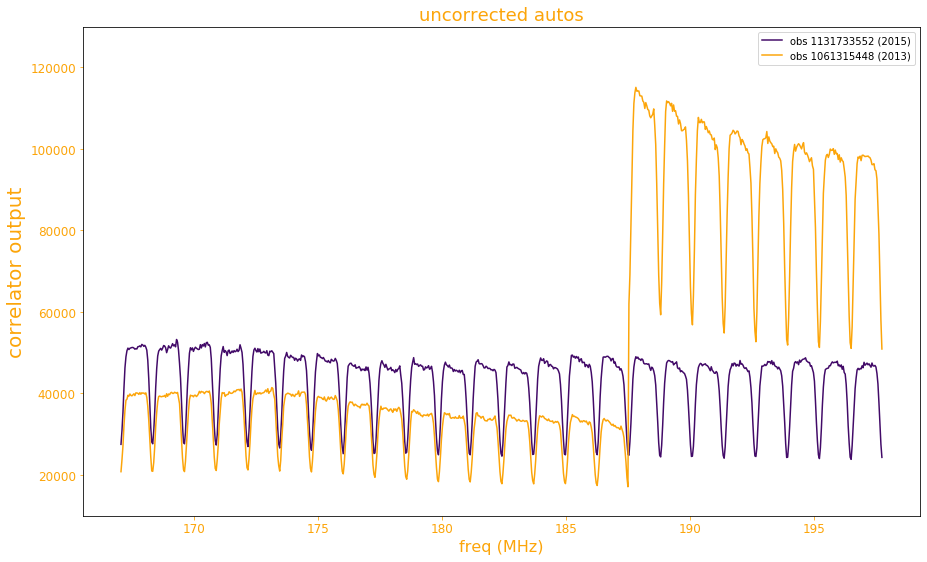
\includegraphics[width=140mm]{uncorr_autos.png}
\caption{Uncorrected 0yy auto-correlations from a 2013 time sample and a 2015 time sample.\label{uncorr_autos}}
\end{figure}
\paragraph{}
The \texttt{pyuvdata} Van Vleck correction implementation was applied to a single time stamp of two observations, 1061315448 from 2013 and 1131733552 from 2015. The first time sample from the second correlator output file for every coarse band was used for each observation. The uncorrected data of the 0yy auto for both samples is shown in figure~\ref{uncorr_autos}. These two samples reflect differences in both digital receiver gain schemes and correlator output files.
\paragraph{}Before the cross-multiply, the correlator casts the quantized integers into floats. As detailed in \cite{beardsley}, this involves division by a factor of 127, which introduces a small error into the data. This error is remedied by casting the data back to integers before storing. After October 2014, data was stored as 32-bit integers with a scaling keyword reflecting the time and frequency integration done in the correlator. Prior to this, the correlator averaged the fine channels to 40 kHz, thus performing a division by 4, and stored the data as floats. To mitigate the errors in this earlier data, the \texttt{pyuvdata} reader for MWA correlator output files casts all data back to integers before processing.
\begin{figure}
\centering{}
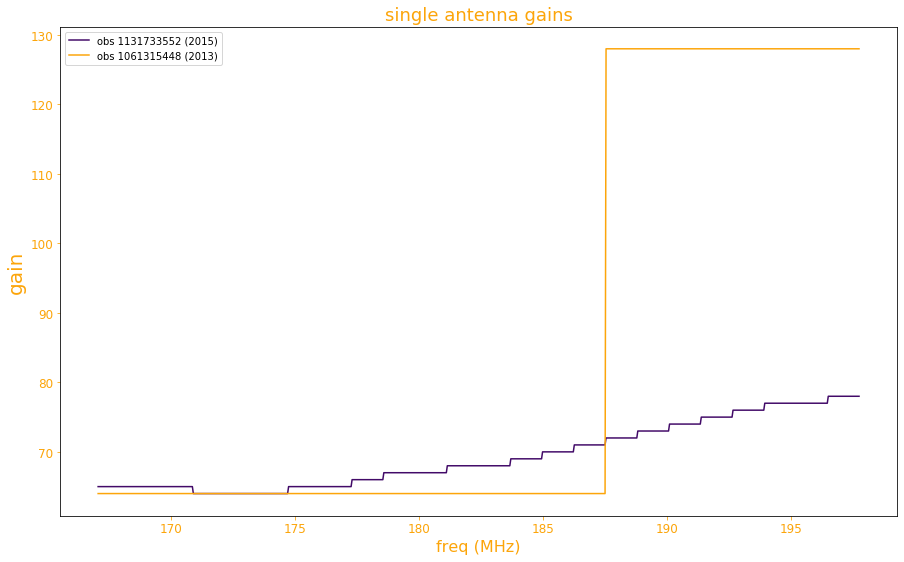
\includegraphics[width=135mm]{gains.png}
\caption{Gains applied to the coarse bands by the MWA digital receivers. These are the gains for a single antenna; in a visibility the gains are squared.\label{gains}}
\end{figure}
\begin{figure}
\centering{}
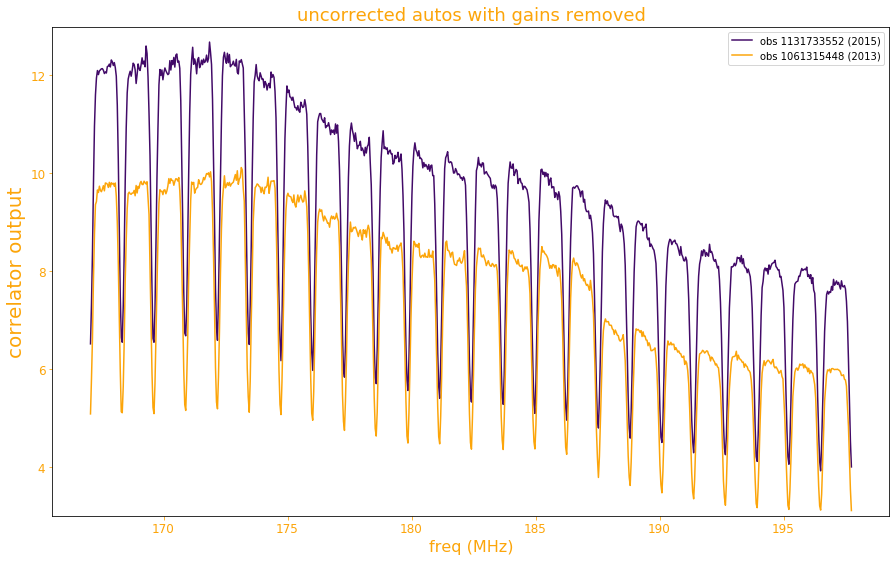
\includegraphics[width=140mm]{uncorr_autos_gains.png}
\caption{Uncorrected auto-correlations with the gains divided out. The gain jump in the 2013 data leaves a discontinuity after the gains are removed.\label{uncorr_autos_gains}}
\end{figure}
\begin{figure}
\centering{}
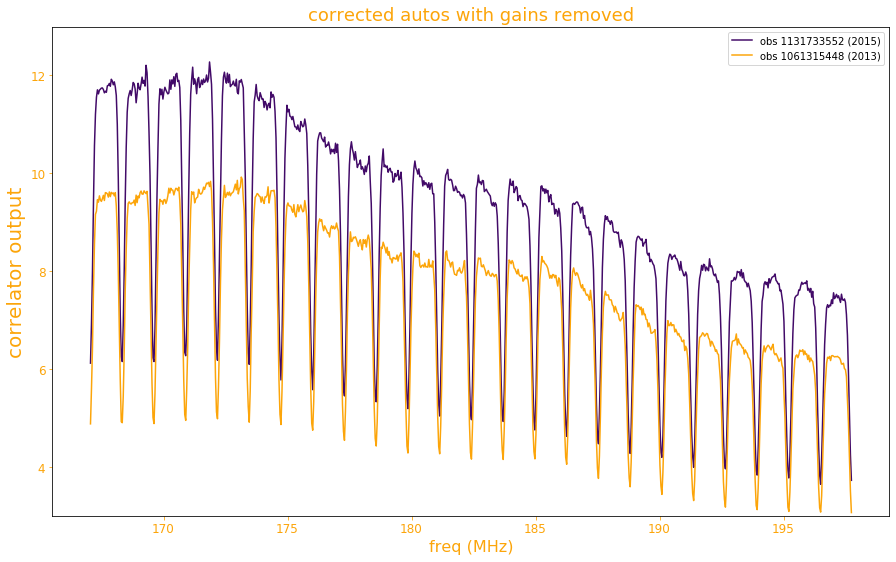
\includegraphics[width=140mm]{corr_autos_gains.png}
\caption{Autocorrelation with the Van Vleck correction applied and then the gains divided out. Applying the Van Vleck correction mitigates the gain jump discontinuity seen in the 2013 data in figure~\ref{uncorr_autos_gains}.\label{corr_autos_gains}}
\end{figure}
\paragraph{}In the 2013 data, the digital receiver gains had a sharp discontinuity across coarse bands, with the 8 highest coarse bands having gains a factor of 2 higher than the lower coarse bands. The gains are plotted in figure~\ref{gains}. Since the gains are applied to each antenna, this leads to a factor of 4 difference in the visibilities. However, simply dividing out the gains does not smooth the coarse bands; a discontinuity is still present as seen in figure~\ref{uncorr_autos_gains}. 
\begin{figure}
\centering{}
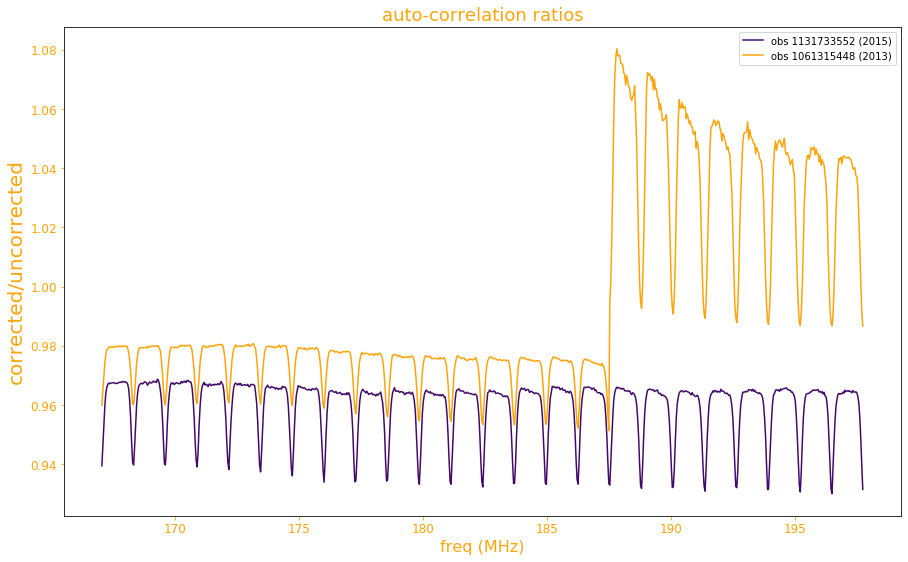
\includegraphics[width=135mm]{auto_ratio.png}
\caption{Ratio between corrected and uncorrected data for an auto-correlation. For 2013 data, the correction decreased values in coarse channels before the digital gain jump and increased values in coarse channels after the digital gain jump. \label{auto_ratio}}
\end{figure}
\begin{figure}
\centering{}
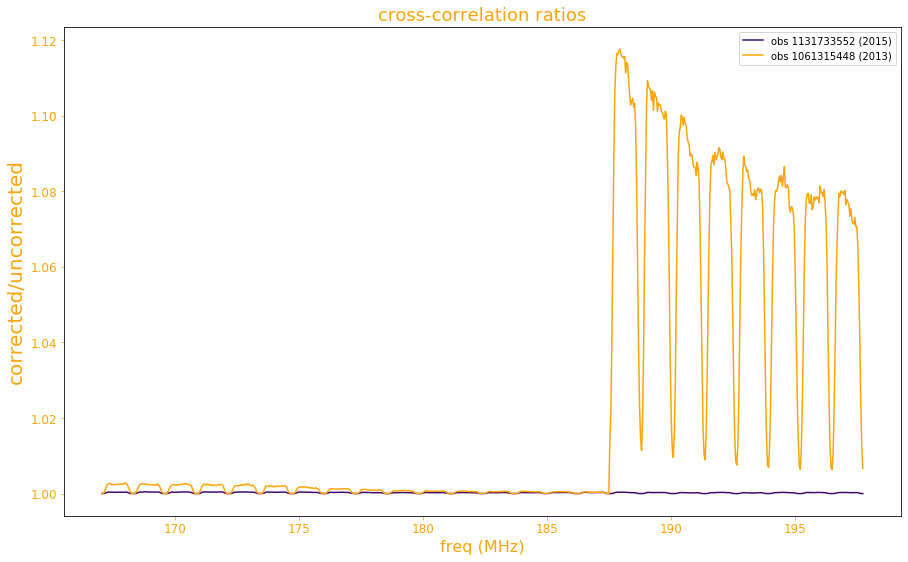
\includegraphics[width=135mm]{cross_ratio.png}
\caption{Ratio between corrected and uncorrected data for a cross-correlation\label{cross_ratio}}
\end{figure}
\begin{figure}
\centering{}
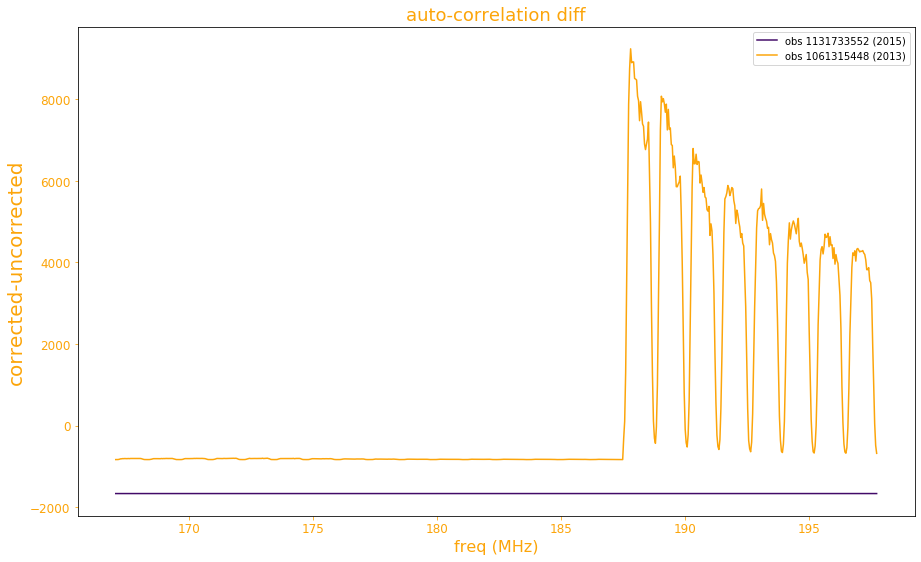
\includegraphics[width=135mm]{auto_diff.png}
\caption{Difference between corrected and uncorrected data for an auto-correlation.\label{auto_diff}}
\end{figure}
\begin{figure}
\centering{}
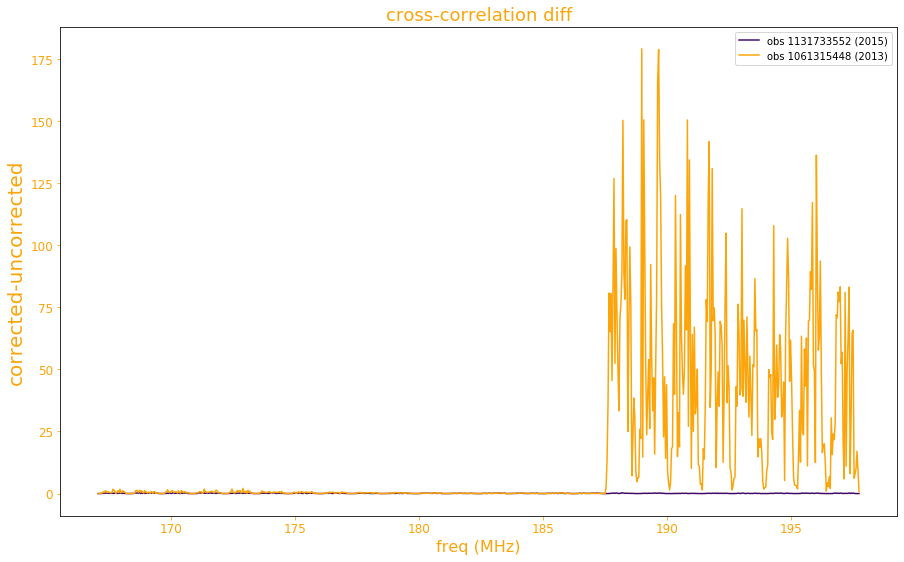
\includegraphics[width=135mm]{cross_diff.png}
\caption{Difference between corrected and uncorrected data for a cross-correlation\label{cross_diff}}
\end{figure}
\paragraph{}
Applying the Van Vleck correction provides some mitigation of the digital gain jump discontinuity seen in the 2013 data, as seen in the initial plot of the 0yy auto (figure~\ref{corr_autos_gains}). Further testing will determine the impacts of the correction on other possible effects of the digital non-linearity. Figures \ref{auto_ratio}, \ref{cross_ratio}, \ref{auto_diff}, \ref{cross_diff} show the ratios and differences between the corrected and uncorrected data for a sample auto-correlation and cross-correlation. For the 2013 auto-correlation, the Van Vleck correction decreased values in the coarse channels before the digital gain jump and increased values in coarse channels after the gain jump. The initial ratio plots show an increase of up to approximately 10\% for coarse channels after the gain jump for both the cross and auto-correlations. The 2015 ratios show more modest changes, with an approximately 3\% decrease in the auto-correlations and cross-correlation ratios very close to 1. More extensive analysis will quantify the range of the ratios and differences across all baselines.
\section{Further work}
\paragraph{}To make implementing the correction feasible on a large scale (correcting a whole night of data, for example) requires a reworking of the cross-correlation correction algorithm. In the meantime, auto-correlations can be corrected and used in testing. A particular area of interest is in removing the coarse band shape introduced by the two PFB stages of the MWA. In \cite{levine_effects} and \cite{levine_math} a shape of the expected coarse band structure was derived. The corrected auto-correlation can be used to test removing this shape. Another interesting effect which might be impacted by removing the digitization non-linearity is the change in the coarse band shapes from night to night. Combining the Van Vleck correction with a deeper analysis of the PFB structures could make previously unusable coarse bands and fine channels available for data analysis. 

\pagebreak
%\nocite{*}
\printbibliography
%\bibliographystyle{apsrmp4-2}
\end{document}